\chapter{Architecture}
\label{chap:implementation}

\section{Basic structure}

To illustrate the functionality of the described algorithm, we have designed a basic application which maintains a data base of images and, for a given query image, can retrieve the best match between
the query and the image set.\\
The basic structure of the application is shown in Figure~\ref{fig:basicStructure}: all the queries are received by the Load Balancer, which acts like a front end processor and distributes in a round-robin fashion the queries to several Map Reduce servers. When these servers receive a query, they distribute it to the associated Image Servers, which contain the descriptors for various sets of images. The Image Servers compute the top $T$ most similar images and then they send it back to the Map Reducer, which extracts the best images from the received responses and sends them back to the Load Balancer. There are several advantages of separating the Map Reducer from the Load Balancer. First of all, it allows load balancing: the Load Balancer can maintain a queue of requests and the Map Reducer with the least work to do can pick it up and process it. Secondly, it allows different types of Image Servers to be tested, by easily inserting and removing the Image Server module.\\
The querying instance type is not particularly important, it can be either a simple web page or a browser extension (e.g. Google Chrome extension).

\tikzstyle{block3} = [rectangle, draw, fill=blue!20, 
    text width=5.5em, text centered, rounded corners, minimum height=3em]
\tikzstyle{line} = [draw, -latex']
\tikzstyle{cloud} = [draw, ellipse,fill=red!20, node distance=1.5cm,
    minimum height=0.5em]
\tikzstyle{block2} = [rectangle, draw, fill=blue!30, 
    text width=5.5em, text centered, rounded corners, minimum height=4em, node distance=3cm]
\tikzstyle{block1} = [rectangle, draw, fill=blue!50, 
    text width=5.5em, text centered, rounded corners, minimum height=3em]
\tikzstyle{cloud2} = [draw, ellipse,fill=green!50, node distance=1.5cm,
    minimum height=0.5em]

\tikzset{
    %Define standard arrow tip
    >=stealth',
    % Define arrow style
    pil1/.style={
           <-,
           thick,
           shorten <=2pt,
           shorten >=2pt,},
    pil2/.style={
           ->,
           thick,
           shorten <=2pt,
           shorten >=2pt,}, 
}

\begin{figure}[H]
\centering

\begin{tikzpicture}[node distance = 2cm, baseline=1em]
    % Place nodes   
    \node [cloud] (query1) {image query};
    \node [cloud, below of = query1] (query2) {image query};
    \node [cloud, below of = query2] (query3) {image query};
    \node [cloud, below of = query3] (query4) {image query};
    \node [cloud, below of = query4] (query5) {image query};
    \node [block1, right of = query3, node distance = 4cm] (loadbalancer) {Load Balancer};
    \node [block2, right of = loadbalancer, node distance = 3cm] (mapreducer1) {MapReducer};
    \node [block2, below of = mapreducer1] (mapreducer2) {MapReducer};
    \node [block2, above of = mapreducer1] (mapreducer3) {MapReducer};
    \node [block3, right of = mapreducer1, node distance = 3cm] (server1) {Image Server};
    \node [block3, below of = server1] (server2) {Image Server};
    \node [block3, above of = server1] (server3) {Image Server};
    \node [block3, below of = server2] (server4) {Image Server};
    \node [block3, above of = server3] (server5) {Image Server};
    % Draw edges
    \path [line] (query1) -- (loadbalancer);
    \path [line] (query2) -- (loadbalancer);
    \path [line] (query3) -- (loadbalancer);
    \path [line] (query4) -- (loadbalancer);
    \path [line] (query5) -- (loadbalancer);
    \path [line] (loadbalancer) -- (mapreducer1);
    \path [line] (loadbalancer) -- (mapreducer2);
    \path [line] (loadbalancer) -- (mapreducer3);
    \path [line] (mapreducer1) -- (server1);
    \path [line] (mapreducer1) -- (server2);
    \path [line] (mapreducer1) -- (server3);
    \path [line] (mapreducer1) -- (server4);
    \path [line] (mapreducer1) -- (server5);
    
\end{tikzpicture}
\caption{Basic structure of service}
\label{fig:basicStructure}
\end{figure}

\section{Load Balancer}

The Load Balancer acts as a classical server. It uses socket communication in order to receive the queries and send them in a round-robin order to the connected Map Reducers. When a response is received from the Map Reducer the Load Balancer sends it back to the entity that has made the given query.\\

\begin{lstlisting}[language=python, caption=Load Balancer pseudocode]
while (true):
  msg = receiveMessage()
  if msg is a Query:
  	send to next Map Reducer
  else if msg is response from Map Reducer:
  	send response back to querying entity
\end{lstlisting}

The command to run the Load Balancer is:
\begin{lstlisting}[language=bash]
make run_load_balancer PORT_FRONT=10000 PORT_BACK=10001
\end{lstlisting}
where PORT_FRONT is the port on which the queries are received and PORT_BACK is the port on which they are passed along to the Map Reducers.

\section{Map Reducer}

The Map Reducer maintains a set of connections with a number of associated Image Servers to which it broadcasts a received query. The Map Reducer waits for the response from the servers (in the meantime it does not process other queries), and combines the received results, by selecting the images with the highest $image\ pair\ score$ from all the images returned by the Image Servers.\\

\begin{lstlisting}[language=python, caption=Map Reducer pseudocode]
while (true):
  query = receiveQueryFromLoadBalancer()
	
  for server in imageServers:
    send(query, server)
  
  for server in imageServers:
    response = receiveResponse(server)
    allResponses.append(response)
	
  sendToLoadBalancer(top T images from allResponses)
\end{lstlisting}

The command to run the Map Reducer is:
\begin{lstlisting}[language=bash]
make run map_reducer PORT_RECV=10001 PORT_PUB=11000 PORT_RSP=11001 CLIENTS=5
\end{lstlisting}

where PORT_RECV is the same as PORT_BACK from the Load Balancer, PORT_PUB is the port on which the query is transmitted to all Image Servers and PORT_RSP is the port used to receive the responses from the Image Servers.
CLIENTS indicated the number of Image Servers connected to the Map Reducer and, implicitly, how many responses must the Map Reducer wait for after publishing a query.

\section{Image Server}

\subsection{Linear Server}
	The first type of server uses the $linear\ algorithm$ described in \nameref{chap:design}. It stores the list of images that form our database and applies the $linear\ algorithm$ a certain query arrives from the Map Reducer.\\

\begin{lstlisting}[language=python, caption=Linear Image Server pseudocode]
def doLinearProcessing(queryImage, imageList):
  for image in imageList:
    allScores.append(computePairImageScore(queryImage, image))
	
    return allScores.sort()
\end{lstlisting}

\subsection{KD-tree Server}
	The second type of server uses the $kdtree\ algorithm$ described in \nameref{chap:design}. At initialization time the server reads a given list of images from our database, computes its descriptors and applies the above mentioned algorithm when a query arrives from the Map Reducer. The resulting KD-tree is maintained in memory throughout the incoming queries and it it used to find the top $T$ most similar images and return them to the Map Reducer.\\

\begin{lstlisting}[language=python, caption=KD-Tree Image Server pseudocode]
def doKDTreeSearch(queryImage, kdTree):
  filteredImages = kdTree.findNearestNeighbors(queryImage)
	
  return doLinearProcessing(queryImage, filteredImages)
\end{lstlisting}

The main problem when storing the descriptors in the KD-tree is in what form to have the images during the computation. We have three possibilities:
\begin{itemize}
 	\item keep them in the original size
	\item resize all the images to a fixed dimension (eg. $400\times300$)
	\item resize all the images to a fixed width and scale the height
\end{itemize}

\subsubsection{Multi-threaded server}
	In order to support a large number of queries on our service, we have implemented the KD-tree Server as a multi-threaded one, each thread being able to process multiple queries.
	The computation of the KD-tree remains on the main thread and, after it is finished, several threads are created with the purpose of responding to queries from the Map Reducers.\\
	As we mentioned before, the Map Reducer is able to process only one query at a time - it receives a query from the Load Balancer, submits it to the Image Servers, and then waits for the responses from these servers.
	So, to take advantage of the multi-threaded implementation of the Image Servers, we have to create multiple Map Reducers, each of them connected to a certain thread in the Image Servers and able to submit and process queries.\\
	Figure~\ref{fig:threads} shows how to Image Servers with 3 threads interact with 3 Map Reducers.\\

\begin{figure}[ht!]
\centering
\begin{tikzpicture}[node distance = 2cm, baseline=1em]
	\matrix(server1)[draw, matrix of nodes, row sep=0.8cm, inner sep=0.3cm, fill=blue!30] {
		Image Server 1 \\
		\node[block1] (T11) {Thread 1};\\
		\node[block1] (T12) {Thread 2};\\
		\node[block1] (T13) {Thread 3};\\
	};
	\matrix(server2)[draw, matrix of nodes, row sep=0.8cm, inner sep=0.3cm, fill=blue!30,
		below of = server1, node distance = 8cm] {
		Image Server 2 \\
		\node[block1] (T21) {Thread 1}; \\
		\node[block1] (T22) {Thread 2};\\
		\node[block1] (T23) {Thread 3};\\
	};
	\node[block2, left of = server1, node distance = 5cm] (mapreducer1) {Map Reducer};
	\node[block2, below of = mapreducer1, node distance = 5cm] (mapreducer2) {Map Reducer};
	\node[block2, below of = mapreducer2, node distance = 5cm] (mapreducer3) {Map Reducer};
	
	\path[line] (mapreducer1) -- (T11);
	\path[line] (mapreducer1) -- (T21);
	\path[line] (mapreducer2) -- (T12);
	\path[line] (mapreducer2) -- (T22);
	\path[line] (mapreducer3) -- (T13);
	\path[line] (mapreducer3) -- (T23);
\end{tikzpicture}
\caption{Image Servers with 3 threads and associated Map Reducers}
\label{fig:threads}
\end{figure}

\subsection{Multiple KD-trees}

Because of the relative constant time of querying a KD-tree, correlated with the fact that this query is an heuristic one (so the quality of the response may get smaller as the size of the KD-tree grows), we have opted to maintain multiple KD-trees in one KD-tree Image Server. We will use the variable
name $R$ to denote the number of KD-trees per Image Server \\
These KD-trees can be searched in a linear fashion, one at a time, or in parallel, with multiple threads (using OpenMP, for example).\\

\begin{lstlisting}[language=python, caption=Multiple KD-Tree Image Server pseudocode]
def doMultipleKDTreeSearch(queryImage, kdTrees):
	for current_kdTree in kdTrees:
		filteredImages.append(current_kdTree.findNearestNeighbors(queryImage))
	
	return doLinearProcessing(queryImage, filteredImages)
\end{lstlisting}

\subsection{Running the Image Server}

The command used to run an Image Server is:

\begin{lstlisting}[language=bash]
make run_images KEY=data_urls START=0 END=25000 TYPE=linear|kdtree IMAGES_KDTREE=2500 NUM_THREADS=1 PORT_FILE=port_file.json COMP=yes|no
\end{lstlisting}

The parameters are:
\begin{itemize}
	\item KEY: the key in the Redis database which stores the urls to be loaded
	\item START, END: the interval of urls from the KEY to be loaded
	\item TYPE: this can be either $linear$ or $kdtree$ depending on the Image Server type
	\item IMAGES_KDTREE: the number of images per KD-tree: the total number of KD-trees per Image Server is computed as the total number of images (END - START + 1) divided by IMAGES_KDTREE
	\item NUM_THREADS: the number of threads per Image Server
	\item PORT_FILE: a JSON file containing the ports used by each thread for communicating with the associated Map Reducer. An example of port file is listed below, with each two consecutive ports representing a communication channel between a thread and a Map Reducer:\\
\begin{lstlisting}[caption=port_file.json]
  ["11000", "11001", "11100", "11101", "11200", "11201"]
\end{lstlisting}
	\item COMP: this can be either $yes$ or $no$, depending if we want to compute the descriptors for the current images, or if we want to load them from the database
\end{itemize}

\section{Technologies}

The majority of our code, Load Balancer, Map Reducer and Image Serves, is written in C++, because of the high computation nature of our problem. For the image processing and associated algorithm we have used OpenCV version 2.4.8 \cite{opencv}.

\subsection{Image Storing}

At first, we stored all our images in a directory on the hard disk, and we maintained a file with all the names of the images we wanted to load in our Image Servers.
This started to be a problem when the number of images started to grow, because keeping all the images in a single directory increased the access time to the respective files (finding, opening and reading from it).\\

We determined that it is better to store only the urls of the images used in out database (not the actual images), the Image Servers downloading an image whenever they need to use it (at initialization time or at query time). The downloading is done using a CURL library for C++ \cite{libcurl}.\\
Also, to avoid computing the SIFT descriptors for all the images every time we start an Image Server we opted to retain those descriptors in our database, and only load them when needed.\\
We maintain a Redis server \cite{redis} on a machine which stores all the urls and the descriptors of the images, and which we can query using a specific C++ library.

\subsection{Process Communication}

For the process communication, we opted to use sockets so that the various servers can reside on different machines.
ZeroMQ sockets \cite{zeromq} looked liked the best option, because of their robustness, small running time, auto-handling of connection failures and multiple types.\\
The ZeroMQ sockets that we used in our service are:
\begin{itemize}
	\item ROUTER-DEALER. We used this pair of sockets to implement the Load Balancer. The ROUTER socket accepts multiple connections, adds a header to the message, to remember which of the connected clients sent it, and forwards it to the DEALER.\\
	The DEALER receives the messages from the ROUTER and distributes them in a round-robin fashion to all the connected clients (which in fact are the Map Reducers). When a reply comes to the DEALER, it forwards it to the ROUTER, which, by inspecting the message's header, identifies the original client and sends it back.
	\item REP. The Map Reducer maintains this type of socket in its communication with the Load Balancer. It allows consecutive operations of receive and send, which suits very well our "receive query - send answer" protocol
	\item PUB-SUB. This pair of sockets forms the connection between a Map Reducer and its associated Image Servers.
	The PUB (publish) socket sends it message to all SUB (subscribed) sockets, making it ideal for the process of map reducing.
	\item PULL-PUSH. This pair of sockets implements the response communication between the Image Server and the Map Reducer. The PUSH (Image Server) sends its response, and the PULL (Map Reducer) receives it.
\end{itemize}

\subsection{Submitting a query and image retrieval}

For submitting a query, we use a JSON-encoded string, which is sent via socket communication to the LoadBalancer, which then forwards it in the above mentioned way. An example of a JSON query string is given below:

\begin{lstlisting}[caption=Query JSON]
{
  "name" : "http://webpa-mp:8080/image/98070.jpg",
  "num_responses" : 10,
  "type_experiment" : 0
}
\end{lstlisting}

The $name$ key represents a url with an associated image, the $num\_responses$ key represents the number of similar images which we want to be returned, and the $type\_experiment$ key represents one of the 3 metrics used (described in \nameref{chap:design}) to be used for extracting the images from the KD-tree.\\

A JSON response string is shown below:

\begin{lstlisting}[caption=Response JSON]
{
  "name": "http://webpa-mp:8080/image/141579.jpg http://webpa-mp:8080/image/223221.jpg http://webpa-mp:8080/image/116303.jpg http://webpa-mp:8080/image/265219.jpg http://webpa-mp:8080/image/216601.jpg http://webpa-mp:8080/image/100891.jpg",
  "scores": "0 18 22 51 79 200 ",
  "time": 1.25,
  "num_responses": 10,
  "type_experiment": 0
}
\end{lstlisting}

The $name$ filed now contains the list of similar images, $scores$ the associated $pair\ image\ scores$ and $time$ the time of the query on the KD-trees The coding and decoding of JSON arrays is done using a special C++ library \cite{jsoncpp}.

\subsection{Web Server}

For the purpose of a web server, which we need for the submission of the queries and local image retrieval, we have used WebPY \cite{webpy}. This server hosts our local images - which can be retrieved by accessing a certain URL, and also is responsable for receiving the queries, forwarding them to the Load Balancer and then generating the HTML for the result page.

\subsection{User interface}

For testing purposes, we have implemented a Google Chrome extension \cite{chromeExtension} which allows a user to select an image from his browser, right click on it, and search our database for similar images. An example of such a search is shown below, where we want to find similar images of the pirate-skull image from the top-right corner: \\

\begin{figure}[ht!]
\centering
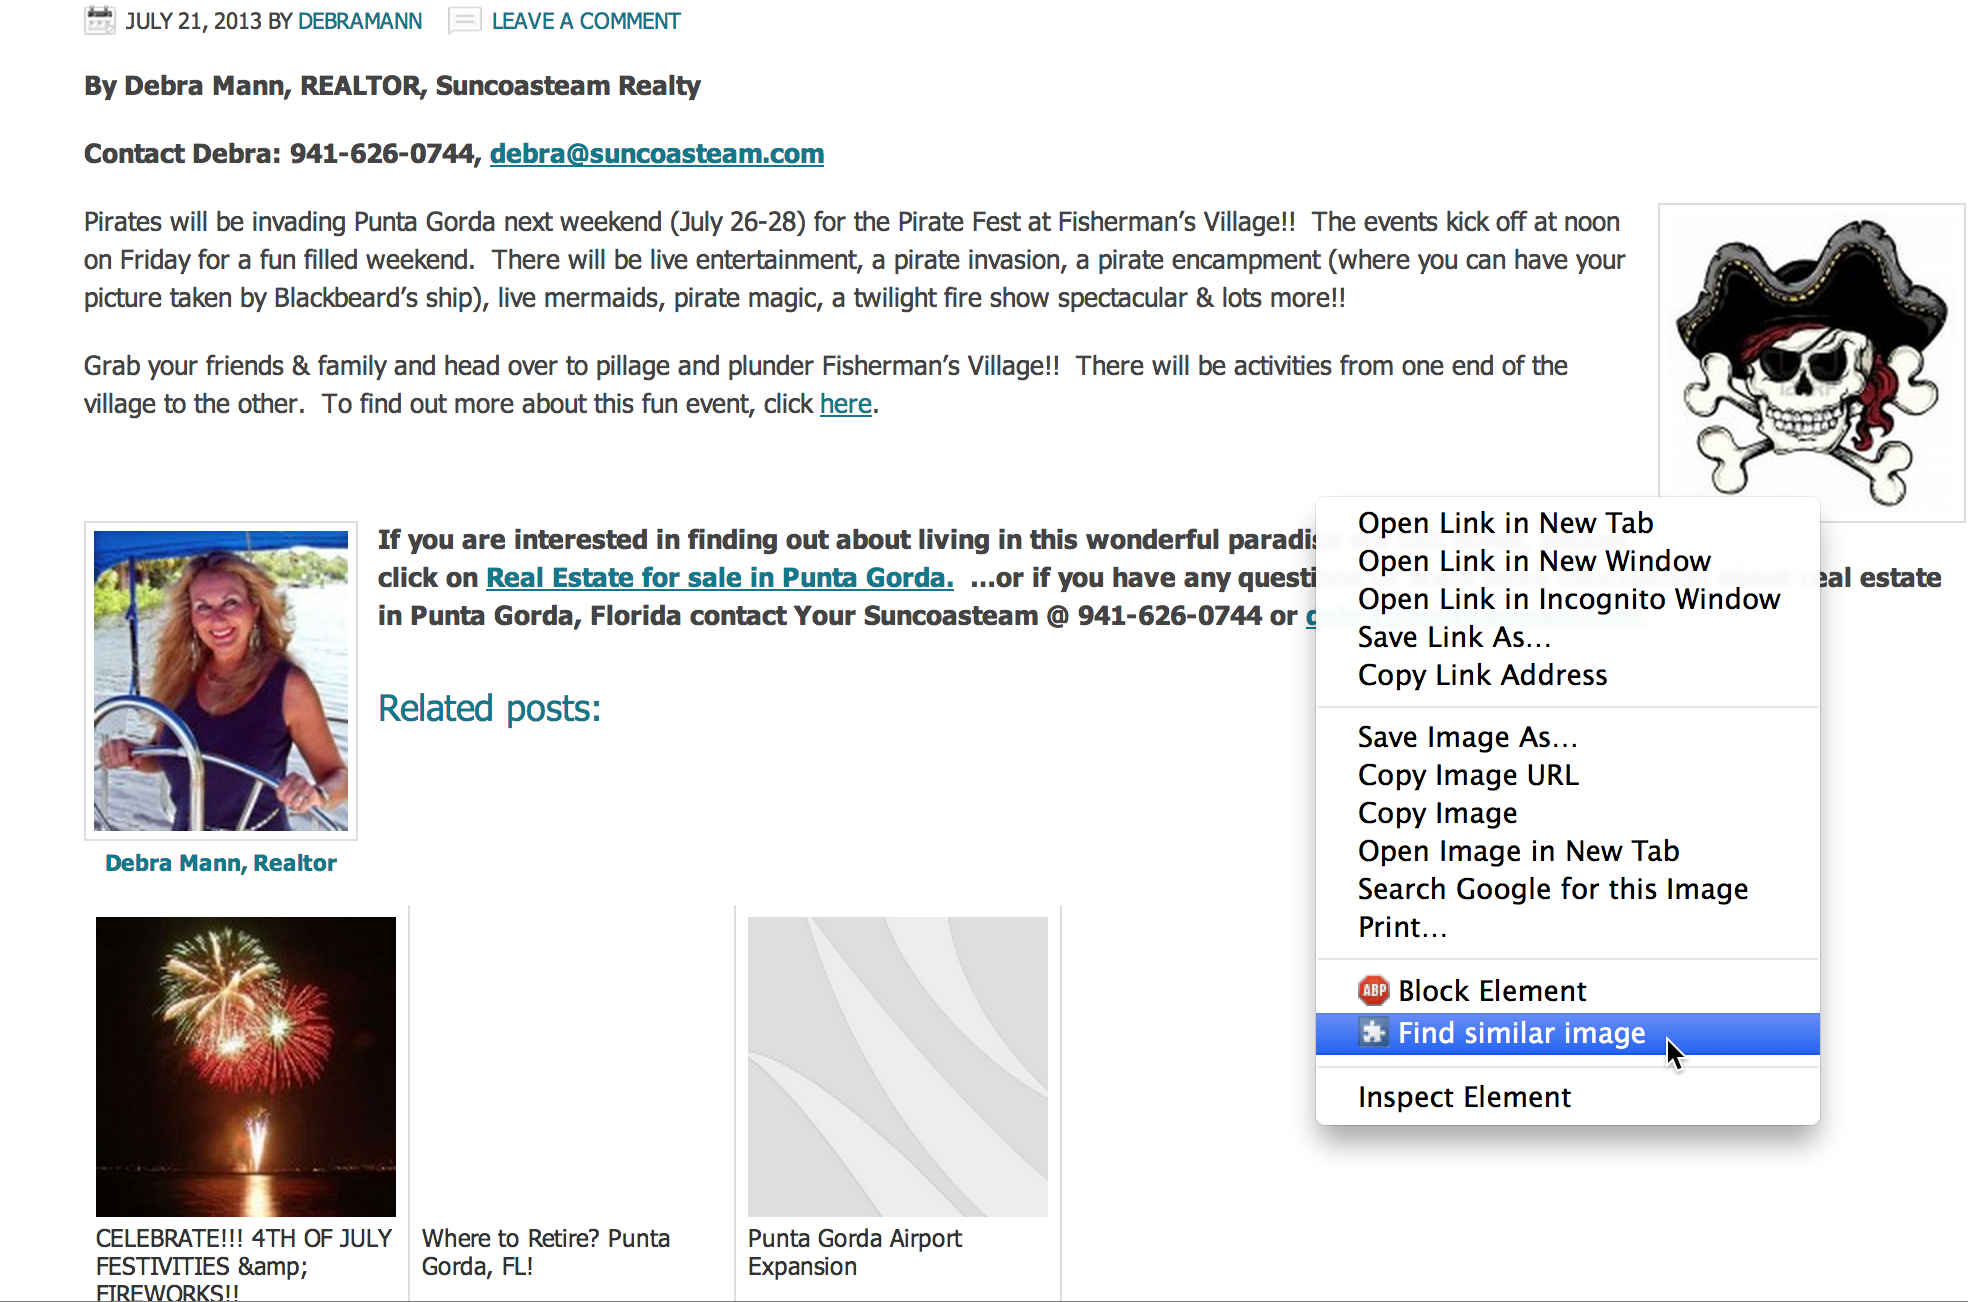
\includegraphics[width=.9\linewidth]{images/extension.png}
\caption{Using the Google Chrome extension}
\end{figure}

The results from the image search can be seen below, where we have the top 3 most similar images from our database, along with the total query time and the associated $pair\ image\ scores$. We have considered a score of less than $50$ represents a highly similar image (marked by a green color), a score less than $100$ a possible similar image (marked by an orange color) and a score higher than $100$ an improbable match (marked with red). 

\begin{figure}[ht!]
\centering
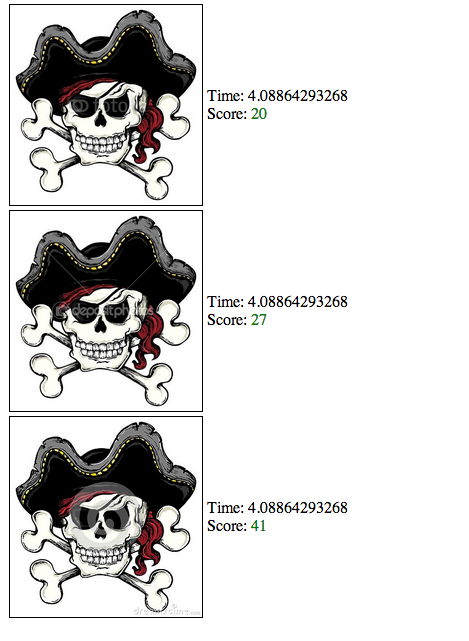
\includegraphics[width=.5\linewidth]{images/extensionResult.png}
\caption{Google Chrome extension result}
\end{figure}


The overall architecture of the entire system is shown in the Figure~\ref{fig:architecture}.
The general workflow of the application is:
\begin{enumerate}
	\item The querying instance (Google Chrome extension) sends the query to the web.py server
	\item The server redirects the query to the Similar Image Service
	\item The service gets the URLs and descriptors from the database
	\item The service may attempt to download images from the web.py server
	\item The server generates the result page, with the found images
\end{enumerate}

\begin{figure}[ht!]
\centering

\begin{tikzpicture}[node distance = 2cm, baseline=1em]
		\node[cloud2] (chrome) {Chrome Extension};
		\node[block2, above of = chrome, node distance = 5cm] (server) {web.py Server}
			edge[pil1] node[auto] {1. Similar Image Query} (chrome.north) ;
		\node[block1, right of = server, node distance = 6cm] (service) {Similar Image Service}
			edge[pil2, bend right = 45] node[auto] {4. Get Images} (server.north) 
			edge[pil1, bend left = 45] node[auto] {2. Send Query} (server.south) ;
		\node[block1, left of = server, node distance = 6cm] (html) {HTML Result Page}
			edge[pil1] node[auto] {5. Show Results} (server.west);
		\node[block1, below of = service, node distance = 7cm] (db) {Redis Database}
			edge[pil1] node[auto] {3. Get URLs and/or descriptors} (service.south);
\end{tikzpicture}
\caption{System architecture}
\label{fig:architecture}
\end{figure}

